\section{两矢量之和}

两个矢量$\bb{u}$和$\bb{v}$的加法可以用两种等价的方式定义\footnote{这两个定义的等价性和唯一性可以从欧氏几何的公设中得到证明:。}。

方式1:三角形法则(图\eqref{fig:1.3}a)。 取代表$\bb{u}$的任何一个箭头,比如$\rr{AB}$。选定后,将有且仅有一个箭头$\rr{BC}$代表$\bb{v}$;$\bb{u}+\bb{v}$被定义为箭头$\rr{AC}$的矢量。如果在使用中希望添加一串矢量(练习1.1),那么这个定义就比较方便,但它无法清晰的体现出矢量加法的交换性。出于对称的原因,最好使用以下定义。

\begin{figure}[htbp]
	\centering
	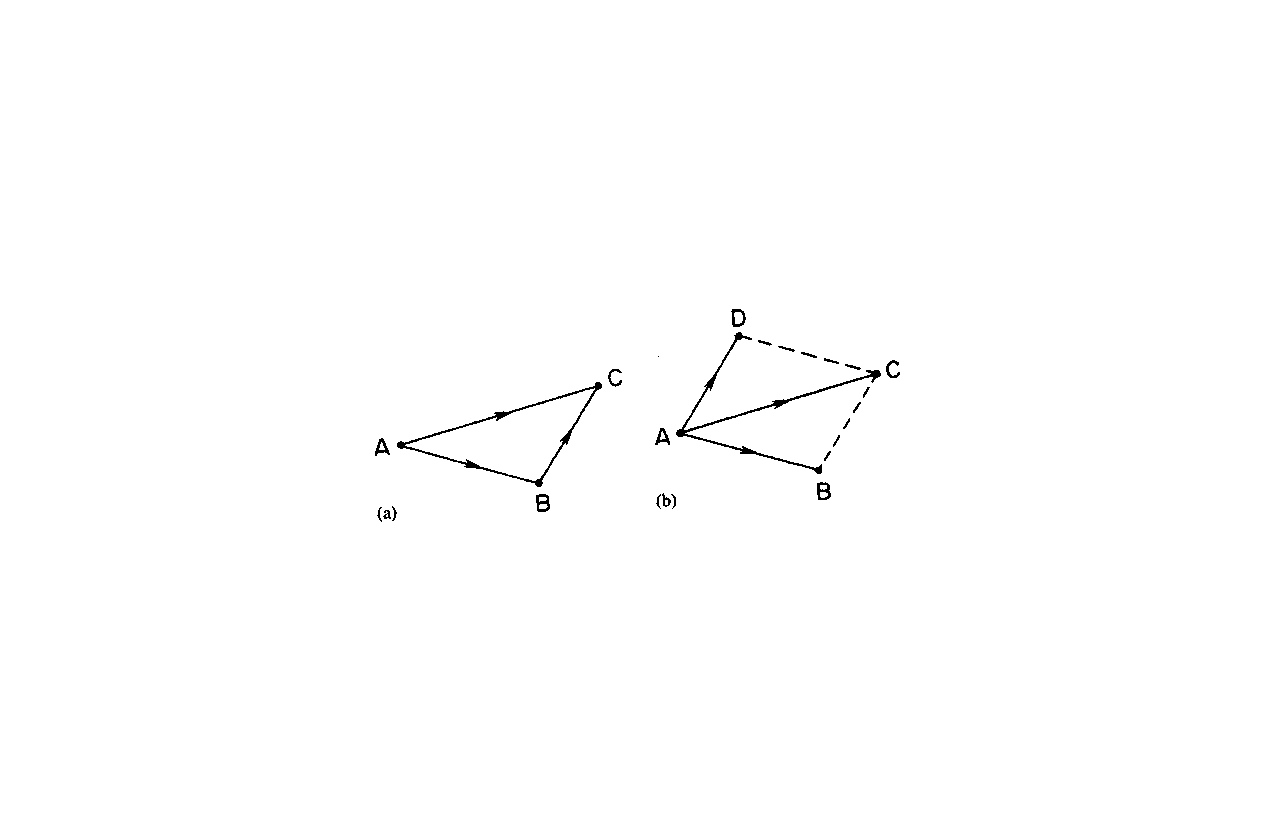
\includegraphics{./image/1.3.pdf}
	\caption{}
	\label{fig:1.3}
\end{figure}

方式2:平行四边形法则(图\eqref{fig:1.3}b)。设$\bb{u}$和$\bb{v}$由任意两个尾端重合的箭头表示,比如$\rr{AB}$和$\rr{AD}$。那么$\bb{u}+\bb{v}$是箭头$\rr{AC}$的矢量,其中$C$是平行四边形的$A$对面的顶点,$\rr{AB}$和$\rr{AD}$为共尾端箭头。

以这种方式添加三个或更多矢量在图形上有点笨拙,但$\bb{u}+\bb{v}+\bb{w}$在三维空间中有以下简洁的解释。令$\bb{u}$、$\bb{v}$和$\bb{w}$由箭头$\rr{AB}$、$\rr{AC}$和$\rr{AD}$表示。 那么对于这个尾端位于$A$,躺在以$\rr{AB}$、$\rr{AC}$和$\rr{AD}$为共端边的平行六面体的对角线上的箭头,$\bb{u}+\bb{v}+\bb{w}$是它的矢量。见练习1.2。